\documentclass[a4paper,twoside]{article}

\usepackage{epsfig}
\usepackage{subfigure}
\usepackage{calc}
\usepackage{amssymb}
\usepackage{amstext}
\usepackage{amsmath}
\usepackage{amsthm}
\usepackage{multicol}
\usepackage{pslatex}
\usepackage{apalike}
\usepackage{SCITEPRESS}
\usepackage[small]{caption}

\subfigtopskip=0pt
\subfigcapskip=0pt
\subfigbottomskip=0pt

\begin{document}

\title{6.867 Machine Learning  \subtitle{Homework 1} }

\maketitle

% **************************************************************************************************
 % Problem 1
% **************************************************************************************************

\section{\uppercase{Implementing Gradient Descent}}

\noindent Gradient descent is an iterative procedure for find a vector that minimize an objective function. Typically, the vector is our parameters and the objective function is the cost function. In each iteration, we find the gradient of the objective function evaluated at the vector and update the vector in the direction of the negative gradient.

\subsection{Basic Gradient Descent}

\noindent To demonstrate the gradient descent algorithm, we began by finding the minimum of two well defined functions with closed form derivatives shown below.

\medskip
\noindent Negative Gaussian:
\begin{equation}
f(x) = - \frac{1}{\sqrt{(2\pi)^n |\Sigma|}} exp[-\frac{1}{2} (x-u)^T\Sigma^{-1}(x-u)]
\end{equation}
\begin{equation}
\frac{\partial f(x)}{\partial x} = -f(x) \Sigma^{-1} (x-u)
\end{equation}

\noindent Quadratic Bowl:
\begin{equation}
f(x) = \frac{1}{2} x^T A x - x^T b
\end{equation}
\begin{equation}
\frac{\partial f(x)}{\partial x} = Ax - b
\end{equation}

\noindent In each iteration, update $x$ according to 
\begin{equation}
x_{t+1} = x_{t} - \eta \bigtriangledown f(x)
\end{equation}
where $\eta$ is the step size. Use the gradient function above to directly compute the gradient at $x$.

\begin{figure}[h]
  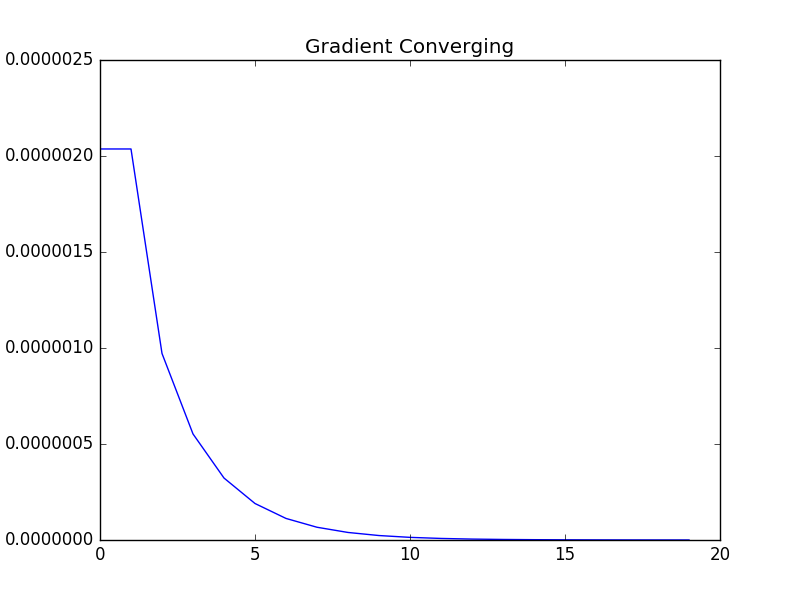
\includegraphics[width=\linewidth]{../Figures/P1/gradient_converging.png}
  \caption{Gradient descent on negative gaussian with step size $\eta = 10^7$. The norm of the gradient is converging to zero.}
  \label{fig:gradient_converging}
\end{figure}

\begin{figure}[h]
  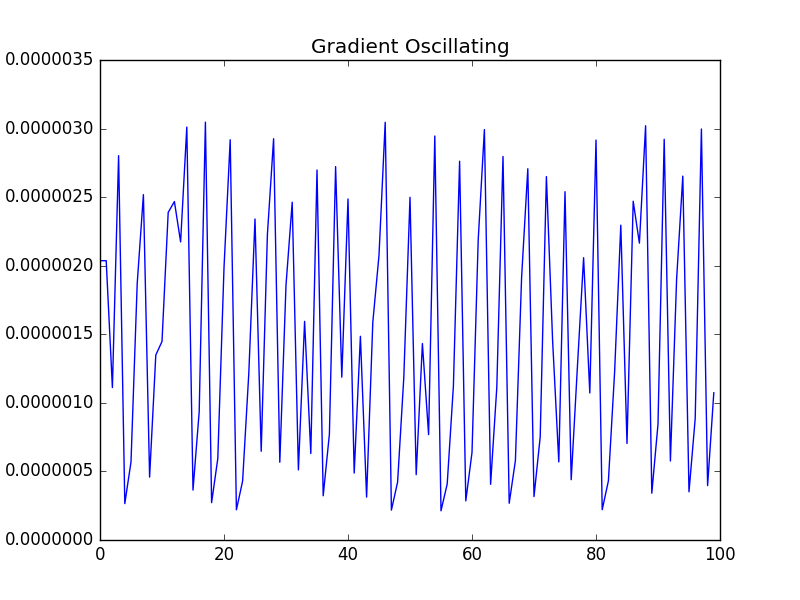
\includegraphics[width=\linewidth]{../Figures/P1/gradient_oscillating.png}
  \caption{Gradient descent on negative gaussian with step size $\eta = 10^7$. The norm of the gradient is oscillating and never converging.}
  \label{fig:gradient_oscillating}
\end{figure}

\begin{figure}[h]
  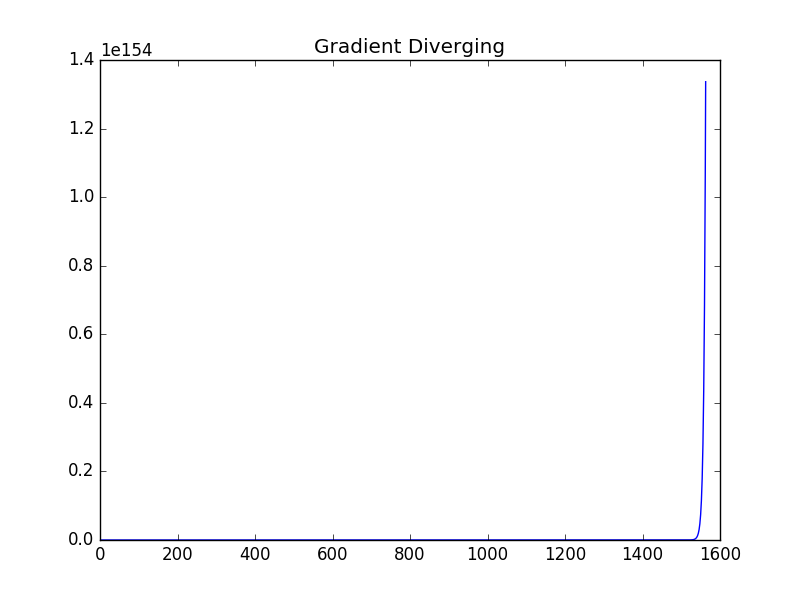
\includegraphics[width=\linewidth]{../Figures/P1/gradient_diverging.png}
  \caption{Gradient descent on negative gaussian with step size $\eta = 10^7$. The norm of the gradient is diverging.}
  \label{fig:gradient_converging}
\end{figure}

The gradient descent algorithm also takes three structural parameters, the starting guess, step size, and convergence criterion. Each affects the end result of the algorithm. The starting guess is important because gradient descent iteratively follows the gradient. Thus it can get stuck in local minimum. By running the algorithm repeated with random initialization, we increase our chance of finding a global minimum. The step size affects convergence behavior of the algorithm. As shown in figures 1-3, if the step size is too small, the algorithm will converge slowly. If the step size is slightly too big, the algorithm will oscillate. If the step size is much too big, the algorithm will actually diverge. The convergence criterion determines for how little change in cost function is it okay to stop. Decreasing this gives greater accuracy but increases runtime.

\subsection{Central Difference Approximation}

For many objective functions, it is impossible to write a closed form gradient function. Thus, use central difference approxiation to approximate the gradient. For each dimension $i$, estimate its partial derivative by 
\begin{equation}
\bigtriangledown_i f(x) = \frac{f(x+d*\hat{\i}) - f(x-d*\hat{\i})}{2d}
\end{equation}
for some small $d$. The larger $d$ is, the more inaccurate the gradient approximation is. We will use $d = 10^{-3}$.

\subsection{Batch vs. Stochastic Gradient Descent}
Now we will use gradient descent to find parameters $\theta$ that minimizes the least squared error objective function
\begin{equation}
J(\theta) = ||X\theta - y||^2
\end{equation}
where each row of $X$ and $y$ is a data sample pair. 

In batch gradient descent, $\theta$ is updated with the gradient of the cost function for the entire training dataset.
Use the gradient function
\begin{equation}
\bigtriangledown_\theta J(\theta) = 2X(X\theta - y)
\end{equation}

Using a step size of $0.01$ and a convergence criterion of $10^-8$, the quadratic bowl function converges in $179$ iterations. The dataset had $100$ points so it took $17900$ point wise gradient evaluations.

In contrast, stochastic gradient descent updates $\theta$ with the gradient of the cost function for each data point. $\theta$ is updated according to 
\begin{equation}
\theta_{t+1} = \theta_t - \eta_t \bigtriangledown_\theta J(\theta_t; x^{(i)}, y^{(i)})
\end{equation}
where $\eta$ is the learning rate and
\begin{equation}
J(\theta_t; x^{(i)}, y^{(i)}) = (x^{(i)T} \theta_t - y^{(i)})^2
\end{equation}
\begin{equation}
\bigtriangledown_\theta J(\theta_t; x^{(i)}, y^{(i)}) = 2(x^{(i)T} \theta_t - y^{(i)}) x^{(i)}.
\end{equation}

 We iterate through the entire dataset for $n$ rounds and for each round, we iterate through the data points in a different order. We converge when the cost between rounds decreases by less than a certain threshold. The stochastic gradient descent took $200000$ pointwise gradient evaluations. The batch gradient descent performed much faster to achieve the same level of convergence but in practice, it is infeasible to compute gradients on large datasets. For such datasets, stochastic gradient descent is the only option.


% **************************************************************************************************
 % Problem 2
% **************************************************************************************************

\section{\uppercase{Linear Basis Function Regression}}

In the supervised learning problem of regression, we are given a set of $n$ data points and $n$ target values and the goal is to find a function that relates $x$ to $y$. We have to do this in such a way that this function generalizes well to unseen values of $x$. Linear Basis Function Regression aims to find the optimal linear combination of basis functions to create a function mapping $x$ to $y$. This linear combination is expressed as a vector of weights for each of these basis functions. These basis functions take the form

\begin{equation}
\phi_i(x) = x^i,  \forall i \in [0,M]
\end{equation}

We evaluated different methods of finding the optimal weight vector, $w$. To do this, we generated 11 points from $y(x) = \cos(\pi x)+1.5 \cos(2 \pi x)$ with some added noise. 

\subsection{Closed Form Solution}

From the textbook, we know the closed form solution for the maximum likelihood weight vector given data values $X$, target values $Y$, and the value of $M$, where $M$ is the highest order polynomial in our polynomial basis. The closed form solution for the maximum likelihood weight vector is
\begin{equation}
(\phi^T \phi)^{-1} \phi^T Y
\end{equation}
where $\phi$ is the design matrix. We tested our solution by plotting the polynomials our models generated against the $11$ data points. As can be seen in figures 4-7, when $M$ is larger the higher polynomial model overfits to the data. We found the optimal $M$ to be $4$.

\begin{figure}[h]
  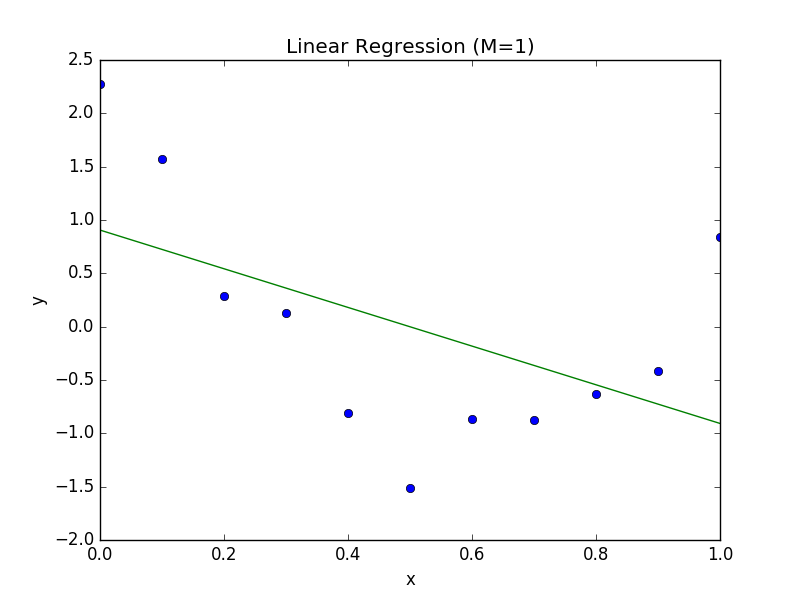
\includegraphics[width=\linewidth]{../Figures/P2/P2.1/M=1.png}
  \caption{}
  \label{fig:gradient_converging}
\end{figure}

\begin{figure}[h]
  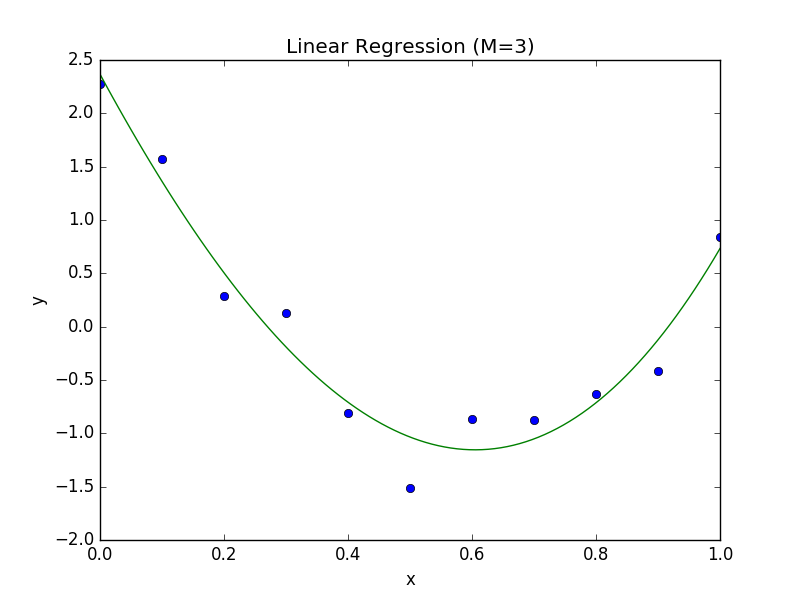
\includegraphics[width=\linewidth]{../Figures/P2/P2.1/M=3.png}
  \caption{}
  \label{fig:gradient_converging}
\end{figure}

\begin{figure}[h]
  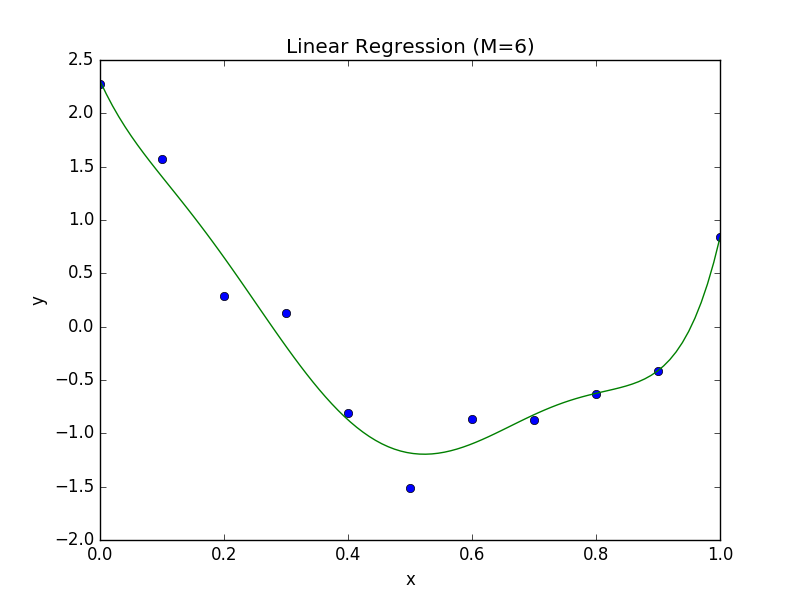
\includegraphics[width=\linewidth]{../Figures/P2/P2.1/M=6.png}
  \caption{}
  \label{fig:gradient_converging}
\end{figure}

\begin{figure}[h]
  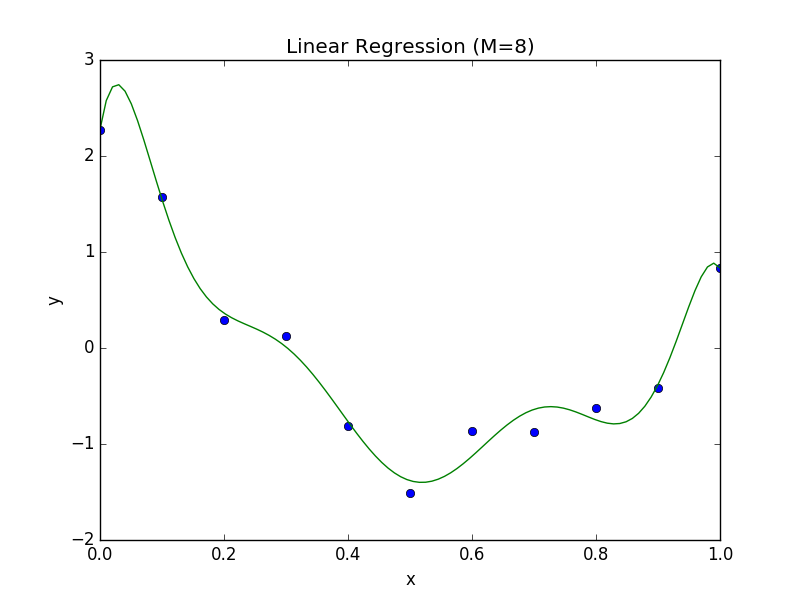
\includegraphics[width=\linewidth]{../Figures/P2/P2.1/M=8.png}
  \caption{}
  \label{fig:gradient_converging}
\end{figure}

\subsection{Objective Function}

The objective function we were trying to minimize was Sum Squared Error. The function and its derivative are 

\begin{equation}
f(x) = \frac{1}{2} \sum_{n=1}^{N} (y_n - w^T \phi(x_n))^2
\end{equation}
\begin{equation}
\bigtriangledown f(x) = \sum_{n=1}^{N} (y_n - w^T \phi(x_n)) \phi(x_n)^T
\end{equation}

. We then used our gradient descent algorithms to find the weight vector that minimized the Sum Squared error. 

\subsection{Batch vs Stochastic Gradient Descent}

We tested different combinations of convergence criterion, step size, initial guess, and M. We found that with batch gradient descent, a step size of $0.1$ achieved the best results. The algorithm achieved lower costs on the cost function and required less iterations than smaller step sizes. Values lower than that would cause the algorithm to converge to a suboptimal value, and values higher than that caused the algorithm to oscillate and fail. We believe that this is because the loss function is less sensitive to changes, allowing for larger step sizes without oscillation. Additionally, we believe that this insensitivity to changes makes it easy for the function to have nearly identical values on successive iterations when the step size is small, causing the algorithm to converge to suboptimal weights. A lower convergence criterion led to better results, but came with the tradeoff of longer convergence times. For example, with $M=4$ and a step size of $.01$, lowering the convergence criterion from $10^{-6}$ to $10^{-7}$ quintupled the number of iterations needed and improved the cost by $.02$. We initialized our parameter vector at random and it didn't affect the converged values of the algorithm. 

With Stochastic Gradient Descent, we found similar trends. Lowering the convergence criterion led to lower costs but more iterations. Increasing the step size (with a max value of 1) generally led to lower costs. A step size of 1 would sometimes give the best results, but other times it caused the algorithm to oscillate and fail. We initialized our parameter vector at random several times and it didn't affect the converged values of the algorithm. 

Batch gradient descent achieved better results, yielding lower costs in nearly every configuration we tested. However, it took a significant number of more iterations than stochastic gradient descent. It often needed more than $10$ times the number of iterations. 

\subsection{Cosine Basis Functions}

We then tested our function for computing the maximum likelihood weight vector by using our prior knowledge about the origin of the data. We used cosine basis functions instead of polynomial ones. The real values of the function that generated the data are $\cos(\pi x)+1.5 \cos(2 \pi x)$, which means its weight vector would be $[1, 1.5]$. Our calculations yielded $[0.7789928, 1.17413213]$. 

% **************************************************************************************************
 % Problem 3
% **************************************************************************************************

\section{\uppercase{Ridge Regression}}

Linear regressions, especially those with sum squared error cost functions, are prone to highly overfit the data. One way to ameliorate this is to introduce a regularization term on your weight vector. Ridge regression punishes weight vectors with large sizes. The parameter $\lambda$ controls how much the size of a vector is penalized. 

\subsection{Closed Form Solution}

We tested different values of $\lambda$ on ridge regressions on a small data set. The tested values of $\lambda$ ranging from $1000$ to $.00001$. With very large $\lambda$ values, the weight vector became the zero vector. In general, as $\lambda$ got smaller, the best fit line produced by the regression was able to fit the data better. This is because when $\lambda = 0$, then it is a normal regression problem with a least squares solution. $\lambda$ effectively works as a bias term, the larger it is, the lower the variance of the weight vector. 

\subsection{Results}

We decided to evaluate the effect $\lambda$ and $M$ have on unseen data. To evaluate this, we trained several models on a training set, $A$, and then used a validation set to determine what models performed the best. We then calculated the error that each of these selected models had on an unseen test set. The models that performed the best on the test set had very low lambda values (between $.000001$ and $.0001$) and had $M = 6$. 

% **************************************************************************************************
 % Problem 4
% **************************************************************************************************

\section{\uppercase{LASSO Regression}}
In some applications, we have reason to believe the underlying function generating the data has sparse weights. In that case, using the $l_1$ norm for regularization, LASSO regression, can perform better than using the $l_2$ norm in ridge regression. To demonstrate this, we have a dataset generated according to 
\begin{equation}
y = w_{true}^T \phi (x) + \epsilon
\end{equation}
$\epsilon$ is some error and $\phi (x)$ is a basis vector defined as 
\begin{equation}
\phi(x) = (x, \sin(0.4 \pi x * 1), ..., \sin(0.4 \pi x * 12))
\end{equation}

$w_{true}^T$ is a vector with sparse weights. We will try to guess them from the training data by perform batch gradient descent to minimize the following objective function for LASSO:
\begin{equation}
\frac{1}{n} \sum_{i=1}^{n} (y^{(i)} - w^T \phi(x^{(i)}))^2 + \lambda \sum_{j=1}^{M} |w_j|
\end{equation}
Different values of $\lambda$ give different weight estimates. The larger $\lambda$ is, the more sparse the weight estimates will be. Unsurprisingly, when $\lambda$ is extremely large, the weights are all zero. These weight estimates can then be plotted by $y = w_{est}^T \phi (x)$ to see how well they performed against the training data. As you can see in figure ?, the lower $\lambda$ is, the more closely the function matches the training data.


Then, from all possible $\lambda, w_{est}$ pairs, we used to validation dataset to choose the pair that performed best. The best $\lambda$ was $10^{-2.55}$ and it yielded an average squared error from the test dataset of $0.0484489$. It is depicted in figure ?.


Using a same procedure with ridge regression, we minimize the objective function
\begin{equation}
\frac{1}{n} \sum_{i=1}^{n} (y^{(i)} - w^T \phi(x^{(i)}))^2 + \lambda \sum_{j=1}^{M} (w_j)^2
\end{equation}
generate weight estimates, and plot them against the sample data. In figure ?, we see weight estimates from different lambdas plotted against the training data.


Figure ? plots the best ridge regression as selected from the validation data set. It is clear the ridge regression performs much worse than LASSO. In fact, the average squared error is $0.635523$, 50\% more than LASSO. LASSO was much better at guessing the sparse true weights.




\begin{figure}[b!]
  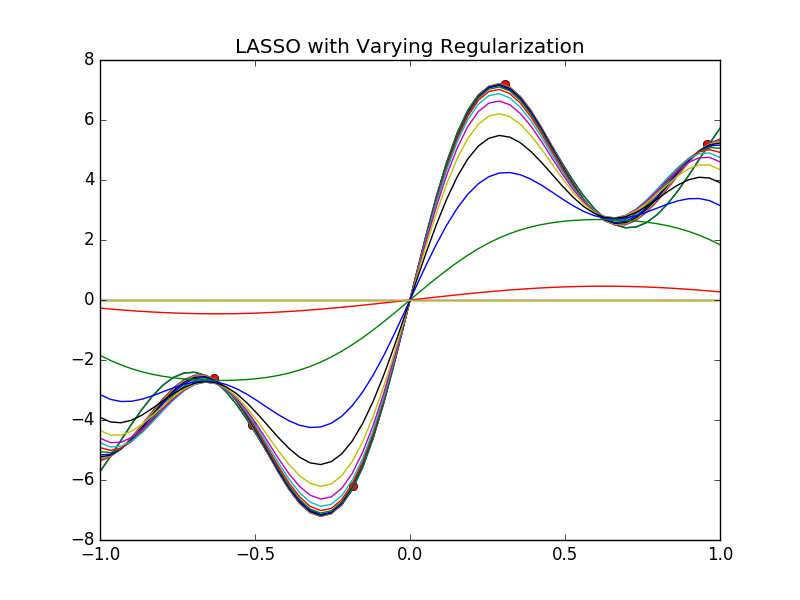
\includegraphics[width=\linewidth]{../Figures/P4/lasso_varying.png}
  \caption{LASSO weight estimates from varying $\lambda$s graphed against training data.}
  \label{fig:lasso_varying}
\end{figure}

\begin{figure}[b!]
  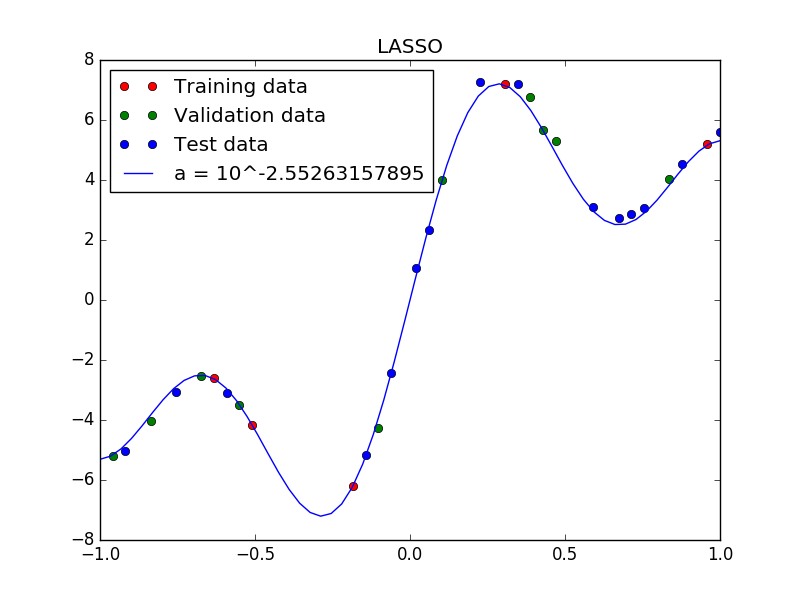
\includegraphics[width=\linewidth]{../Figures/P4/lasso_best.png}
  \caption{Best LASSO weight estimate.}
  \label{fig:lasso_best}
\end{figure}

\begin{figure}[b!]
  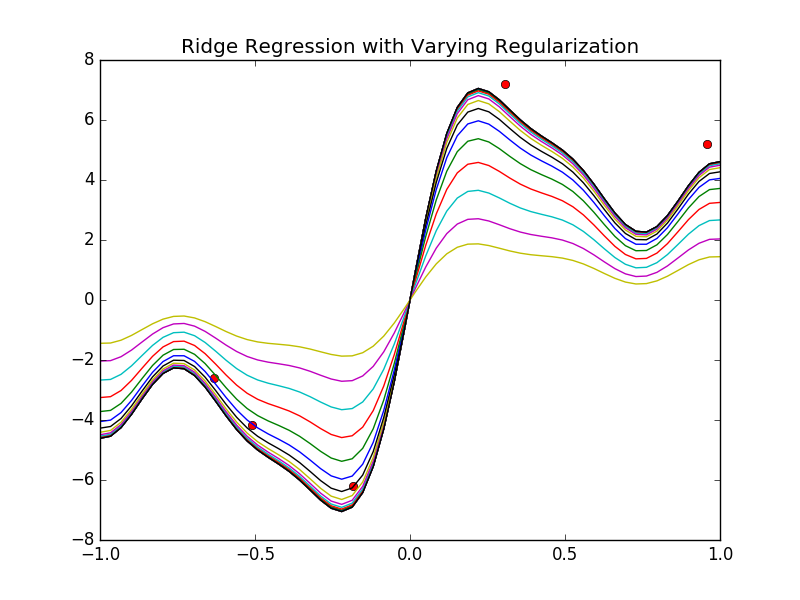
\includegraphics[width=\linewidth]{../Figures/P4/ridge_varying.png}
  \caption{Ridge regression weight estimates from varying $\lambda$s graphed against training data.}
  \label{fig:ridge_varying}
\end{figure}

\begin{figure}[b!]
  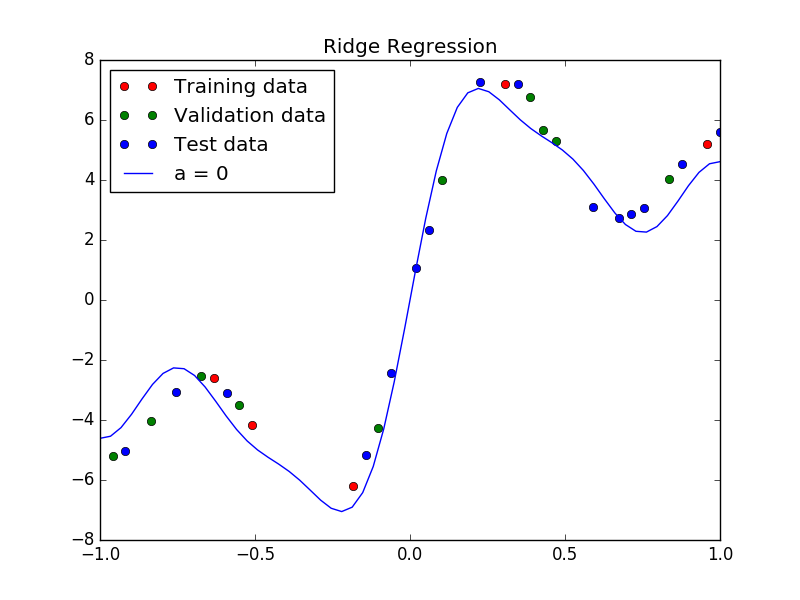
\includegraphics[width=\linewidth]{../Figures/P4/ridge_best.png}
  \caption{Best ridge regression weight estimate.}
  \label{fig:ridge_best}
\end{figure}

\vfill
\end{document}

